\documentclass{article}
\usepackage{amsmath}
\usepackage{amssymb}
\usepackage{graphicx}
\usepackage{fontspec}
\setmainfont[Mapping=tex-text]{STSong}
\usepackage{listings}
\usepackage{hyperref}
\lstset{
frame=single
}
\hypersetup{colorlinks = true,
	    linkcolor = black,
	    urlcolor = blue,
            citecolor = blue}
\title{Final Homework}
\date{苑闻 2200010833}
\begin{document}
\maketitle
求解Stokes方程:\\
\begin{equation}
\label{eq6}
\left\{
\begin{aligned}
-\Delta \vec u + \nabla p &= \vec F, &(x, y) \in (0, 1) \times (0, 1)\\
{\rm div} \vec u &= 0, &(x, y) \in (0, 1) \times (0, 1)\\
\end{aligned}
\right.
\end{equation}
边界条件
\begin{align*}
\frac{\partial u}{\partial \vec n}&=b, y=0,&\frac{\partial u}{\partial \vec n}=t, y=1 \\
\frac{\partial v}{\partial \vec n}&=l, x=0,&\frac{\partial v}{\partial \vec n}=r, x=1 \\
u&=0, x=0,1,&v=0, y=0,1
\end{align*}
其中$\vec u = (u,v)$为速度, p为压力, $\vec F = (f,g)$为外力, $\vec n$为外法向方向\\
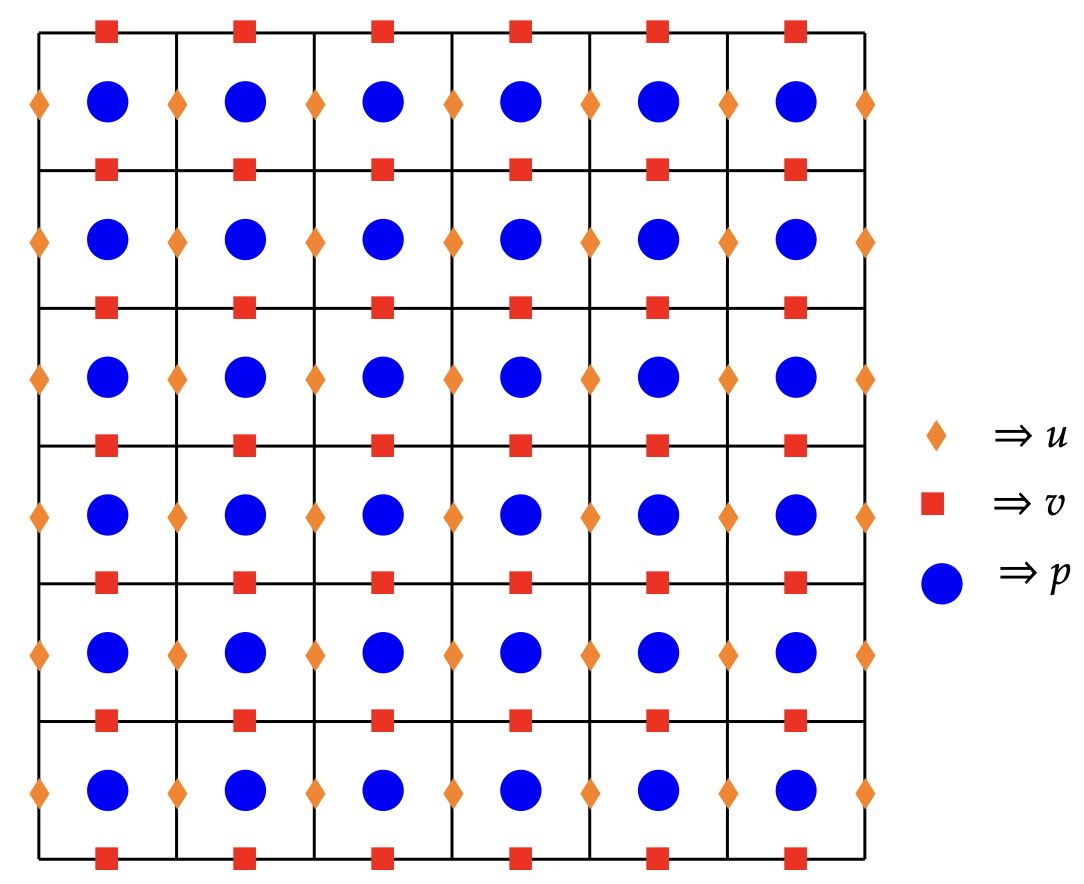
\includegraphics[scale=0.5]{image/form.png}\\
stokes方程数值形式为($h=\frac{1}{N}$):
\begin{align*}
-\frac{u_{i+1,j-\frac{1}{2}}-2u_{i,j-\frac{1}{2}}+u_{i-1,j-\frac{1}{2}}}{h^2}
-\frac{u_{i,j+\frac{1}{2}}-2u_{i,j-\frac{1}{2}}+u_{i,j-\frac{3}{2}}}{h^2}
+\frac{p_{i+\frac{1}{2},j-\frac{1}{2}}-p_{i-\frac{1}{2},j-\frac{1}{2}}}{h}
&= f_{i,j-\frac{1}{2}}\\
-\frac{v_{i-\frac{1}{2},j+1}-2v_{i-\frac{1}{2},j}+v_{i-\frac{1}{2},j-1}}{h^2}
-\frac{v_{i+\frac{1}{2},j}-2v_{i-\frac{1}{2},j}+v_{i-\frac{3}{2},j}}{h^2}
+\frac{p_{i-\frac{1}{2},j+\frac{1}{2}}-p_{i-\frac{1}{2},j-\frac{1}{2}}}{h}
&= g_{i-\frac{1}{2},j}\\
\frac{u_{i,j-\frac{1}{2}}-u_{i-1,j-\frac{1}{2}}}{h}
+\frac{v_{i-\frac{1}{2},j}-v_{i-\frac{1}{2},j-1}}{h} &= 0
\end{align*}
边界条件的数值形式为:
\begin{align*}
-\frac{u_{i+1,\frac{1}{2}}-2u_{i,\frac{1}{2}}+u_{i-1,\frac{1}{2}}}{h^2}
-\frac{u_{i,\frac{3}{2}}-u_{i,\frac{1}{2}}}{h^2}
+\frac{p_{i+\frac{1}{2},\frac{1}{2}}-p_{i-\frac{1}{2},\frac{1}{2}}}{h}
&= f_{i,\frac{1}{2}}+\frac{b_{i,0}}{h}\\
-\frac{u_{i+1,N-\frac{1}{2}}-2u_{i,N-\frac{1}{2}}+u_{i-1,N-\frac{1}{2}}}{h^2}
+\frac{u_{i,N-\frac{1}{2}}-u_{i,N-\frac{3}{2}}}{h^2}
+\frac{p_{i+\frac{1}{2},N-\frac{1}{2}}-p_{i-\frac{1}{2},N-\frac{1}{2}}}{h}
&= f_{i,N-\frac{1}{2}}+\frac{t_{i,N}}{h}\\
-\frac{v_{\frac{1}{2},j+1}-2v_{\frac{1}{2},j}+v_{\frac{1}{2},j-1}}{h^2}
-\frac{v_{\frac{3}{2},j}-v_{\frac{1}{2},j}}{h^2}
+\frac{p_{\frac{1}{2},j+\frac{1}{2}}-p_{\frac{1}{2},j-\frac{1}{2}}}{h}
&= g_{\frac{1}{2},j}+\frac{l_{0,j}}{h}\\
-\frac{v_{N-\frac{1}{2},j+1}-2v_{N-\frac{1}{2},j}+v_{N-\frac{1}{2},j-1}}{h^2}
+\frac{v_{N-\frac{1}{2},j}-v_{N-\frac{3}{2},j}}{h^2}
+\frac{p_{N-\frac{1}{2},j+\frac{1}{2}}-p_{N-\frac{1}{2},j-\frac{1}{2}}}{h}
&= g_{N-\frac{1}{2},j}+\frac{r_{N,j}}{h}\\
u_{0,j-\frac{1}{2}}=u_{N,j-\frac{1}{2}}=v_{i-\frac{1}{2},0}=v_{i-\frac{1}{2},N}=0
\end{align*}
将第k次迭代的$u_{i,j-\frac{1}{2}}$记为$u^k_{i,j}$, 
$v_{i-\frac{1}{2},j}$记为$v^k_{i,j}$, 
$p_{i-\frac{1}{2},j-\frac{1}{2}}$记为$p^k_{i,j}$\\
则我们需要解线性方程:
$$
\begin{bmatrix}
	A & B\\
	B^T & 0
\end{bmatrix}
\begin{bmatrix}
	U\\
	P
\end{bmatrix}
=
\begin{bmatrix}
	F\\
	0
\end{bmatrix}
$$
\section{DGS+Vcycle}
\subsection{Algorithm}
\subsubsection{单次DGS迭代}
\subsubsection*{Gauss迭代更新速度分量}
stokes方程的Gauss迭代可以写成:
\begin{align*}
-\frac{u^k_{i+1,j}-2u^{k+1}_{i,j}+u^{k+1}_{i-1,j}}{h^2}
-\frac{u^k_{i,j+1}-2u^{k+1}_{i,j}+u^{k+1}_{i,j-1}}{h^2}
+\frac{p^k_{i+1,j}-p^k_{i,j}}{h}
&= f_{i,j-\frac{1}{2}}\\
-\frac{v^k_{i,j+1}-2v^{k+1}_{i,j}+v^{k+1}_{i,j-1}}{h^2}
-\frac{v^k_{i+1,j}-2v^{k+1}_{i,j}+v^{k+1}_{i-1,j}}{h^2}
+\frac{p^k_{i,j+1}-p^k_{i,j}}{h}
&= g_{i-\frac{1}{2},j}
\end{align*}
边界条件的Gauss迭代可以写成:
\begin{align*}
-\frac{u^k_{i+1,1}-2u^{k+1}_{i,1}+u^{k+1}_{i-1,1}}{h^2}
-\frac{u^k_{i,2}-u^k_{i,1}}{h^2}
+\frac{p^k_{i+1,1}-p^k_{i,1}}{h}
&= f_{i,\frac{1}{2}}+\frac{b_{i,0}}{h}\\
-\frac{u^k_{i+1,N}-2u^{k+1}_{i,N}+u^{k+1}_{i-1,N}}{h^2}
+\frac{u^{k+1}_{i,N}-u^{k+1}_{i,N-1}}{h^2}
+\frac{p^k_{i+1,N}-p^k_{i,N}}{h}
&= f_{i,N-\frac{1}{2}}+\frac{t_{i,N}}{h}\\
-\frac{v^k_{1,j+1}-2v^{k+1}_{1,j}+v^{k+1}_{1,j-1}}{h^2}
-\frac{v^k_{2,j}-v^{k+1}_{1,j}}{h^2}
+\frac{p^k_{1,j+1}-p^k_{1,j}}{h}
&= g_{\frac{1}{2},j}+\frac{l_{0,j}}{h}\\
-\frac{v^k_{N,j+1}-2v^{k+1}_{N,j}+v^{k+1}_{N,j-1}}{h^2}
+\frac{v^{k+1}_{N,j}-v^{k+1}_{N-1,j}}{h^2}
+\frac{p^k_{N,j+1}-p^k_{N,j}}{h}
&= g_{N-\frac{1}{2},j}+\frac{r_{N,j}}{h}\\
u^{k+1}_{0,j}=u^{k+1}_{N,j}
=v^{k+1}_{i,0}=v^{k+1}_{i,N}=0
\end{align*}
\subsubsection*{对每个内部单元(i,j)计算散度残量}
\begin{align*}
r_{i,j} = -\frac{u^{k+1}_{i,j}-u^{k+1}_{i-1,j}}{h}
-\frac{v^{k+1}_{i,j}-v^{k+1}_{i,j-1}}{h}
\end{align*}
令$delta = r_{i,j}h/4$
\subsubsection*{更新内部单元速度}
\begin{align*}
u^{k+2}_{i-1,j} = u^{k+1}_{i-1,j}-\delta,
u^{k+2}_{i,j} = u^{k+1}_{i,j}+\delta\\
v^{k+2}_{i,j-1} = v^{k+1}_{i,j-1}-\delta,
v^{k+2}_{i,j} = v^{k+1}_{i,j}+\delta
\end{align*}
\subsubsection*{更新内部单元压力}
\begin{align*}
p^{k+2}_{i,j} &= p^k_{i,j}+r_{i,j},\\
p^{k+2}_{i+1,j} &= p^k_{i+1,j}-r_{i,j}/4,
p^{k+2}_{i-1,j} = p^k_{i-1,j}-r_{i,j}/4,\\
p^{k+2}_{i,j+1} &= p^k_{i,j+1}-r_{i,j}/4,
p^{k+2}_{i,j-1} = p^k_{i,j-1}-r_{i,j}/4,
\end{align*}
\subsubsection*{更新边界单元和顶点单元}
与前面类似, 只是将分子的4换成3和2
\subsubsection{Vcycle}
Vcycle算法框架如下 (求解$Ax=b$):\\
1) 每一轮开始时, 如果是最上层循环, 以上一轮得到的$x_0$作为初始值, 否则用0作为初始值
2) 先做$\nu_1$次DGS得到$x_0$\\
3) 再计算当今误差$b_0=b-Ax_0$, 对其做一次限制算子降低维数得到$b_1$\\
4) 重复Vcycle, 近似求解$Ax_1=b_1$\\
5) 对求解到的$x_1$做一次提升算子得到$x_2$\\
6) 更新$x_0<-x_0+x_2$
7) 再做$\nu_2$次DGS得到$x_0$\\
8) 回溯\\
以下为课堂上的限制和提升算子:\\
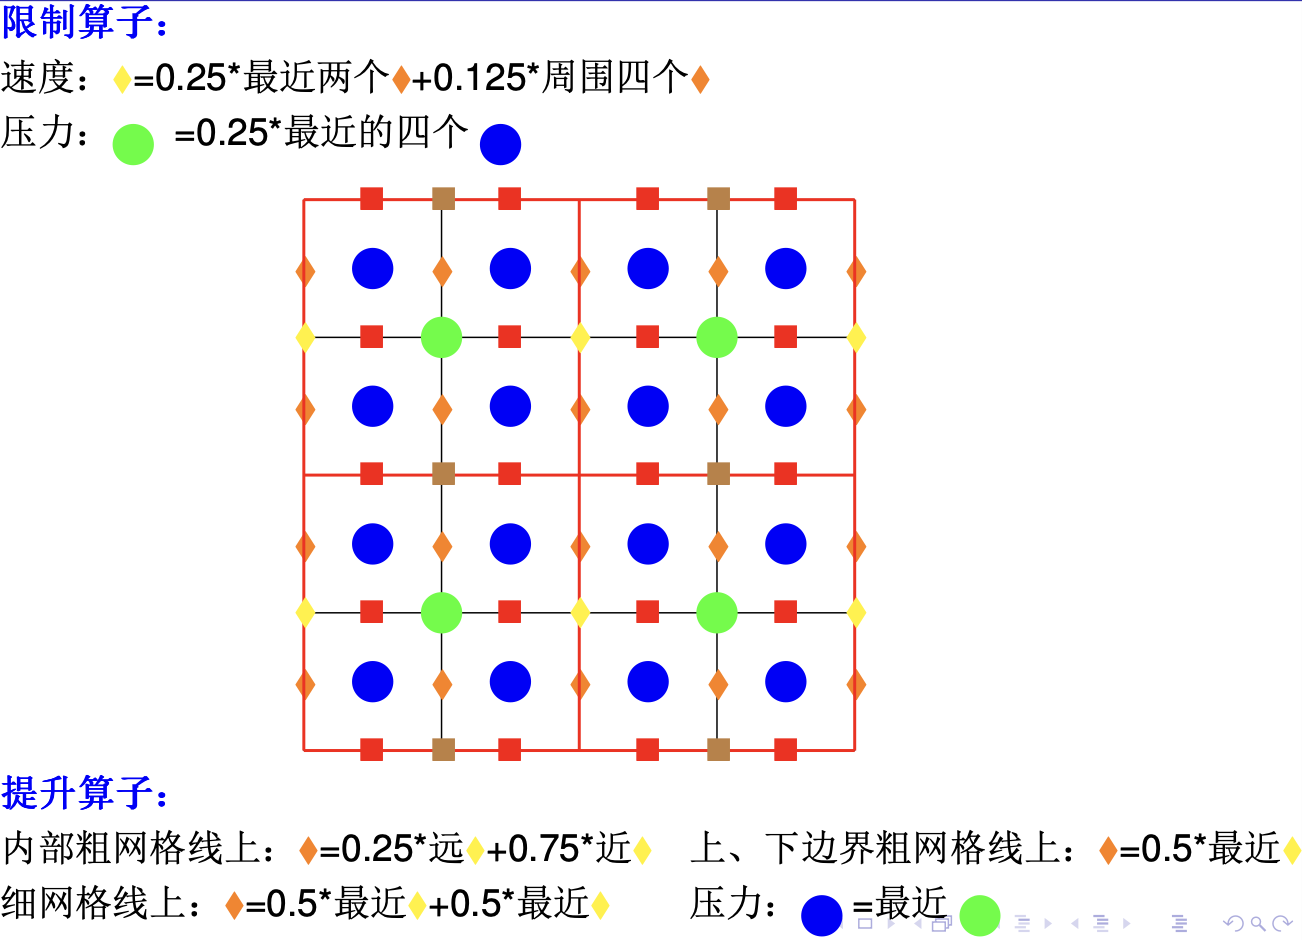
\includegraphics[scale=0.5]{image/updownclass.png}\\
以下为作业pdf中新加上的限制和提升算子:\\
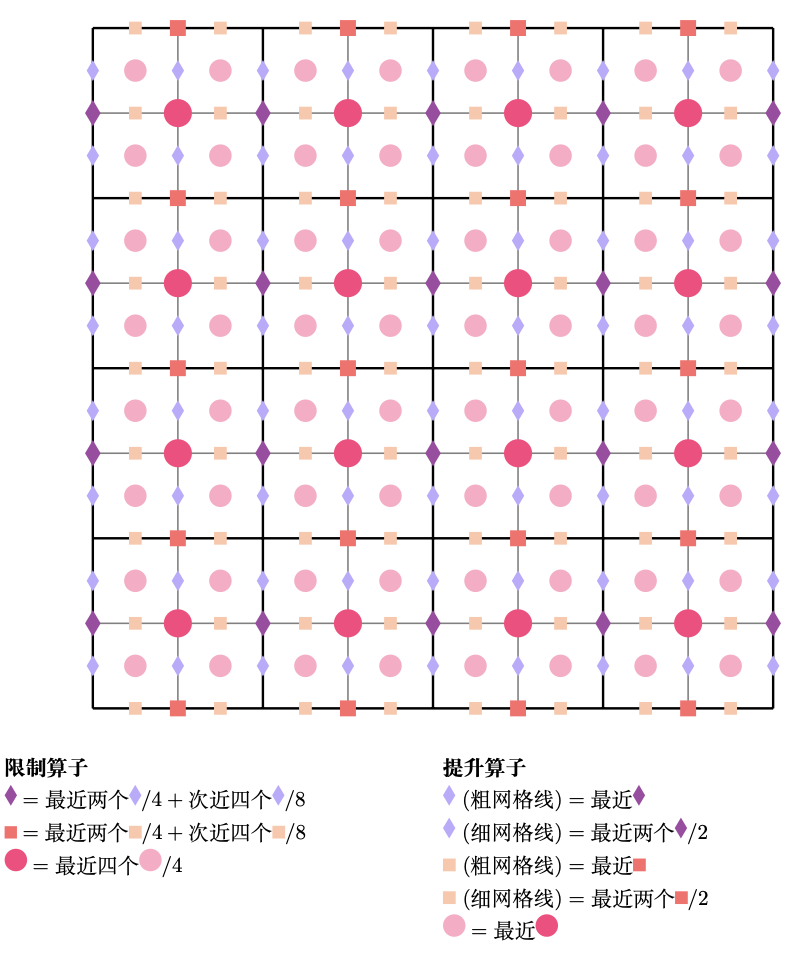
\includegraphics[scale=0.5]{image/updownpdf.png}\\
\subsection{Implementation}
具体函数见code里的README.md\\
\subsection{Result}
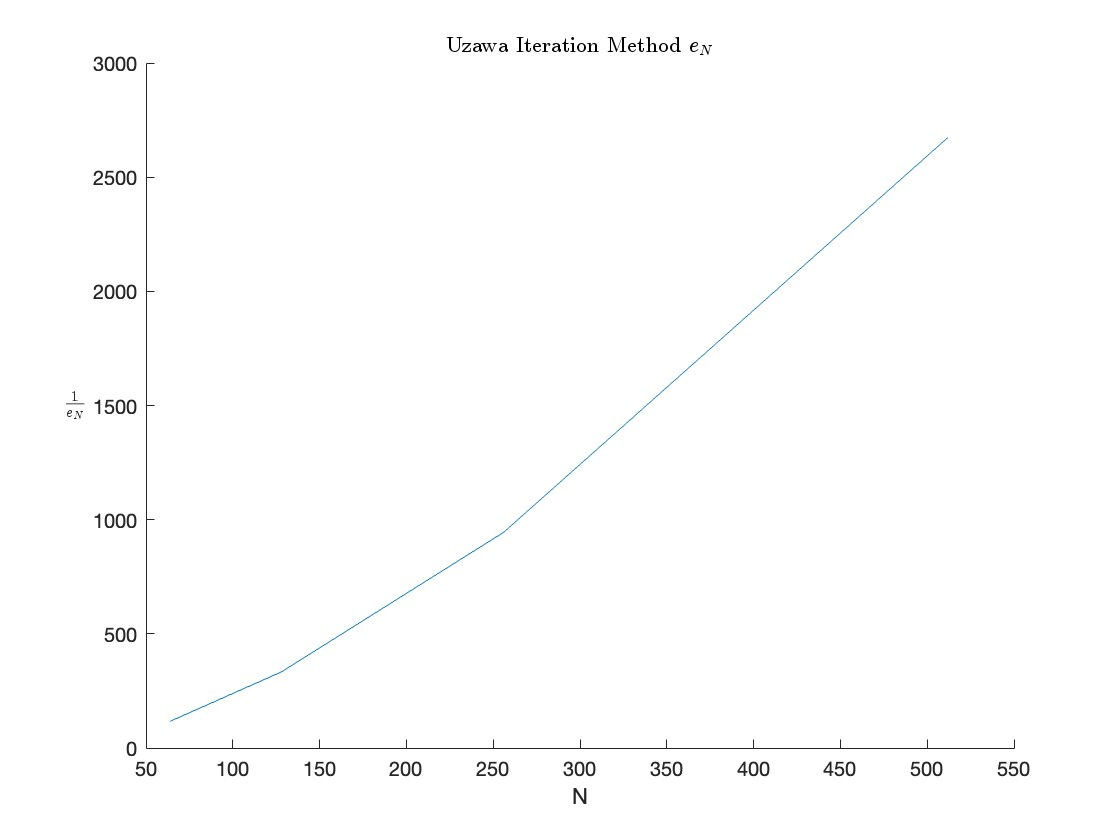
\includegraphics[scale=0.3]{image/DGS.jpg}\\
\begin{tabular}{llll}
N & time & $e_N$ & steps \\ 
\hline 
64 & 0.14275 & 0.0085233 & 6 \\ 
128 & 0.12871 & 0.0030007 & 6 \\ 
256 & 0.57573 & 0.0010587 & 7 \\ 
512 & 2.4236 & 0.00037395 & 7 \\ 
1024 & 18.5366 & 0.00013215 & 7 \\ 
2048 & 94.1432 & 4.6709e-05 & 7 \\ 
\hline 
\end{tabular}\\
由图易见$e_N=O(\frac{1}{N})$
\section{Uzawa Iteration Method + CG}
\subsection{Algorithm}
算法框架如下:\\
1) 每一轮开始时, 用共轭梯度法求解$AU_{k+1}=F-BP_k$\\
2) 然后对压力进行更新$P_{k+1}=P_k+\alpha(B^TU_{k+1})$\\
3) 判断误差是否小于允许的值, 从而判断是否回到第一步\\
上面$\alpha$选取为\\
$$
\alpha_{\star}=\frac{2}{\lambda_{min}{B^TA^{-1}B}+\lambda_{max}{B^TA^{-1}B}}
$$
\subsection{Implementation}
具体函数见code里的README.md\\
\subsection{Result}
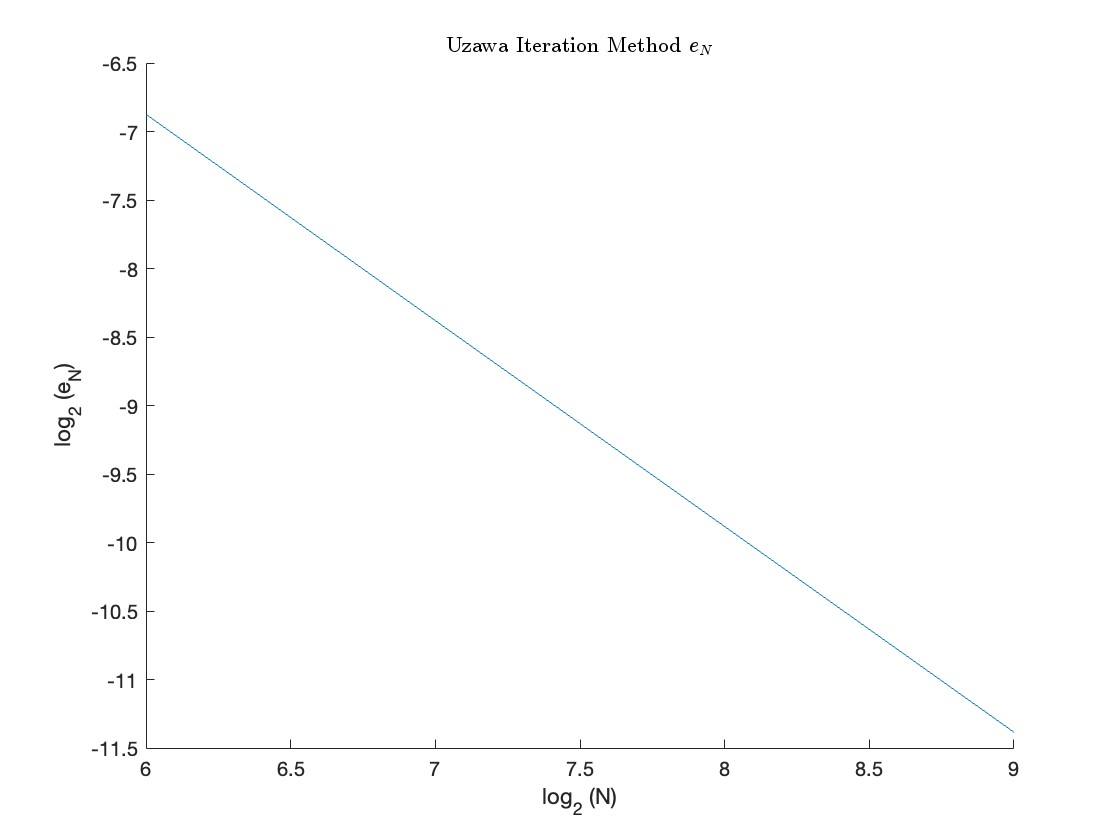
\includegraphics[scale=0.3]{image/UIM.jpg}\\
\begin{tabular}{lll}
N & time & $e_N$ \\ 
\hline 
64 & 0.13661 & 0.0085233 \\ 
128 & 0.47766 & 0.0030007 \\ 
256 & 4.7065 & 0.0010587 \\ 
512 & 27.9452 & 0.00037395 \\ 
\hline 
\end{tabular}\\
由图易见$e_N=O(\frac{1}{N})$
\section{Inexact Uzawa Iteration Method + Vcycle}
\subsection{Algorithm}
算法框架如下:\\
1) 每一轮开始时, 用预条件共轭梯度法近似求解$AU_{k+1}=F-BP_k$, 
使用$M=A$作为预条件矩阵, 求解预条件方程的时候使用Vcycle方法求解\\
2) 然后对压力进行更新$P_{k+1}=P_k+\alpha(B^TU_{k+1})$\\
3) 判断误差是否小于允许的值, 从而判断是否回到第一步\\
上面$\alpha$选取为\\
$$
\alpha_{\star}=\frac{2}{\lambda_{min}{B^TA^{-1}B}+\lambda_{max}{B^TA^{-1}B}}
$$
近似求解$AU_{k+1}=F-BP_k$得到的$\hat{U}_{k+1}$需要满足若定义$$
\delta_k = A\hat{U}_{k+1}-F+BP_k
$$
则
$$
||\delta_k||_2 \leq \tau||B^T\hat{U}_k||
$$
\subsection{Implementation}
具体函数见code里的README.md\\
\subsection{Result}
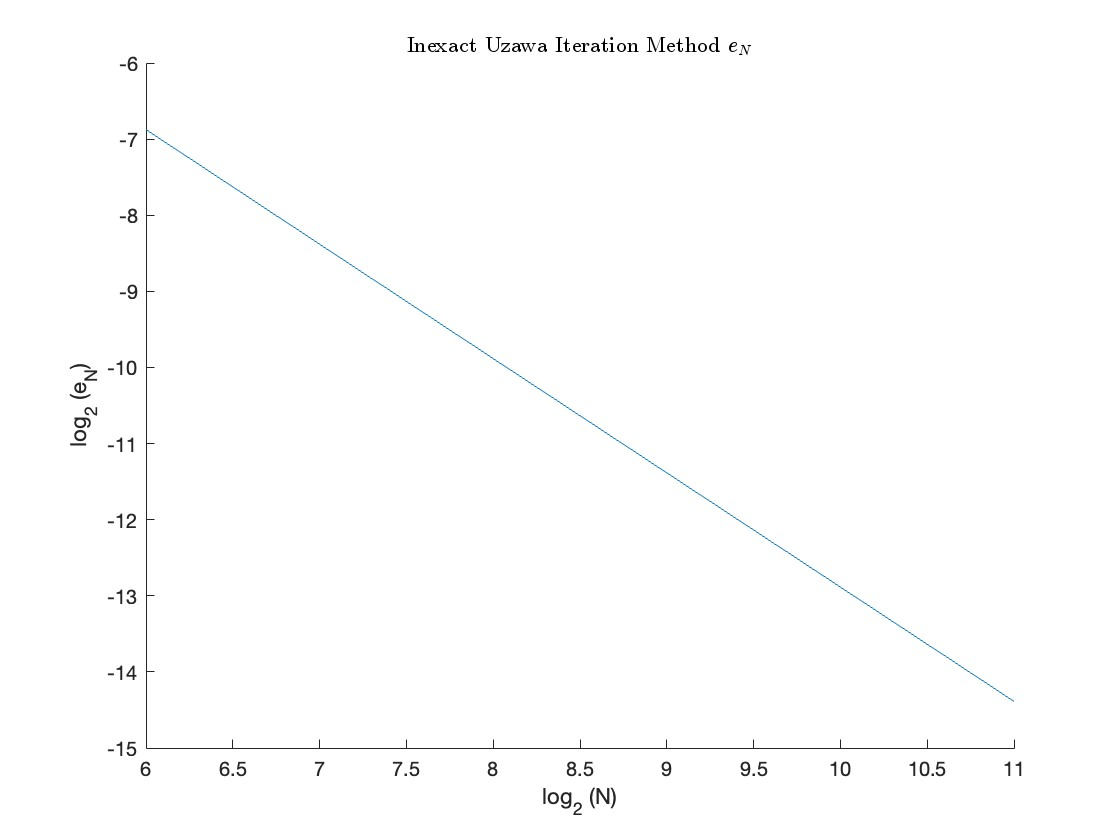
\includegraphics[scale=0.3]{image/IUIM.jpg}\\
\begin{tabular}{llll}
N & time & $e_N$ & steps \\ 
\hline 
64 & 0.065143 & 0.0085233 & 4 \\ 
128 & 0.25165 & 0.0030007 & 4 \\ 
256 & 0.99247 & 0.0010587 & 4 \\ 
512 & 4.0304 & 0.00037395 & 4 \\ 
1024 & 24.4011 & 0.00013212 & 4 \\ 
2048 & 129.3766 & 4.6674e-05 & 4 \\ 
\hline 
\end{tabular}\\
由图易见$e_N=O(\frac{1}{N})$
\end{document}
